\documentclass[border=8pt,tikz]{standalone}
\usepackage{tikz}
\usepackage{amsmath}
\usepackage[T1]{fontenc}
\usepackage{lmodern}
\usetikzlibrary{arrows.meta,positioning,calc,shapes.geometric,decorations.pathreplacing,backgrounds,fit,patterns}

\definecolor{bg}{HTML}{0A0A0A}
\definecolor{maroon}{HTML}{800020}
\definecolor{maroonLight}{HTML}{B03050}
\definecolor{maroonDeep}{HTML}{4A0014}
\definecolor{accent}{HTML}{E8C547}
\definecolor{text}{HTML}{F5F5F5}
\definecolor{muted}{HTML}{A0A0A0}
\definecolor{cardbg}{HTML}{1A1A1A}
\definecolor{blockbg}{HTML}{220812}

\begin{document}
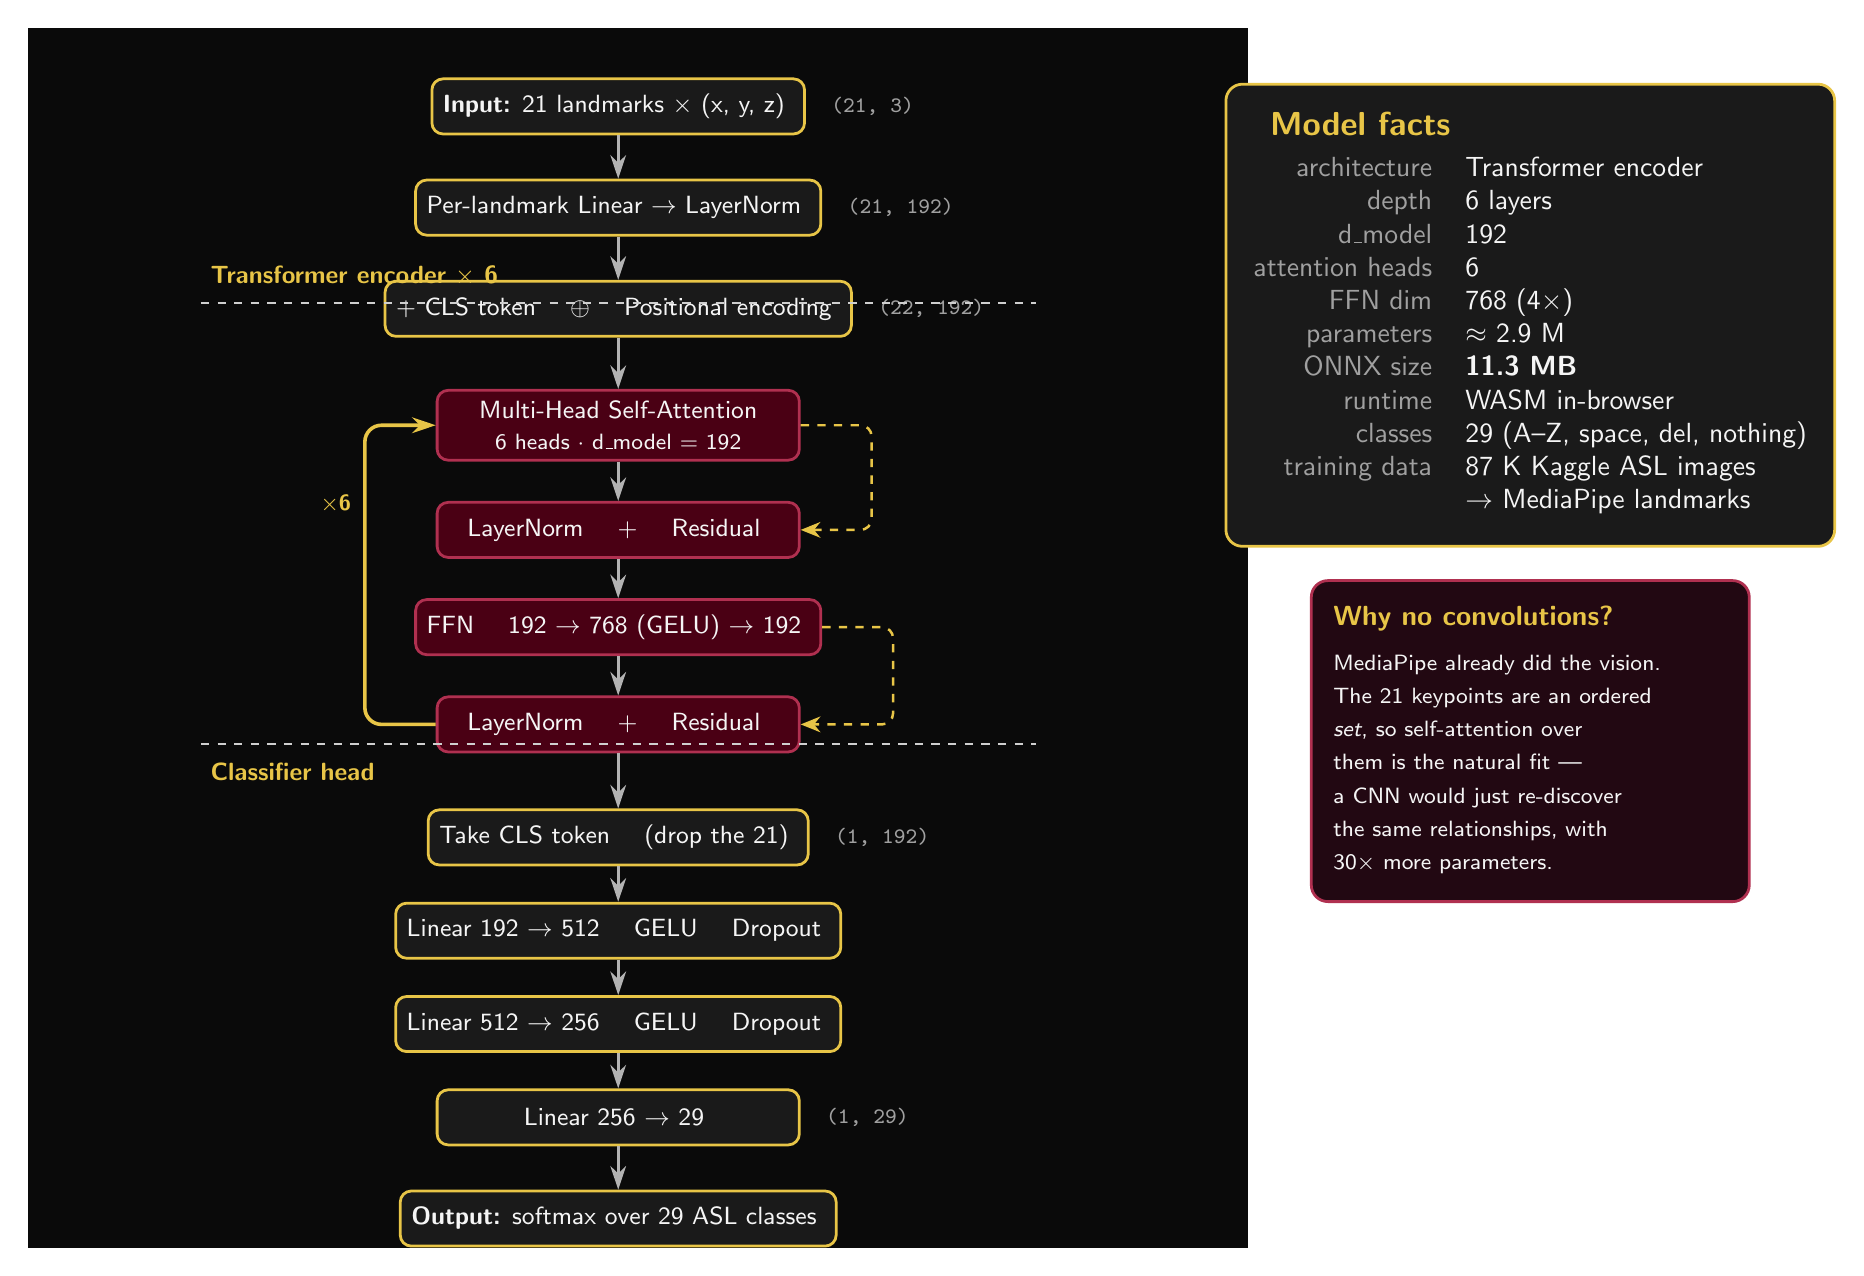
\begin{tikzpicture}[
    font=\sffamily,
    every node/.style={text=text},
    block/.style={
        rectangle, rounded corners=4pt,
        draw=maroonLight, line width=1pt,
        fill=blockbg,
        minimum width=4.6cm, minimum height=0.7cm,
        align=center, font=\sffamily\small,
        inner sep=4pt,
    },
    embed/.style={block, draw=accent, fill=cardbg},
    attn/.style={block, draw=maroonLight, fill=maroonDeep},
    head/.style={block, draw=accent, fill=cardbg},
    arrow/.style={-{Stealth[length=3mm,width=2mm]}, line width=1pt, draw=muted!80},
    addarrow/.style={-{Stealth[length=2.5mm,width=2mm]}, line width=0.9pt, draw=accent, dashed},
    sectionlabel/.style={font=\sffamily\bfseries\small, text=accent},
    divider/.style={dashed, draw=muted!50, line width=0.7pt},
    dimnote/.style={font=\sffamily\footnotesize\ttfamily, text=muted, anchor=west},
]

% Background
\fill[bg] (-7.5,-12) rectangle (8,3.5);

% =============================================================
% LEFT COLUMN: forward pass through the network
% =============================================================

% Input
\node[embed] (input) at (0,2.5) {
    \textbf{Input:} 21 landmarks $\times$ (x, y, z)
};
\node[dimnote] at ($(input.east)+(0.2,0)$) {(21, 3)};

\node[embed, below=0.55cm of input] (proj) {
    Per-landmark Linear $\rightarrow$ LayerNorm
};
\node[dimnote] at ($(proj.east)+(0.2,0)$) {(21, 192)};

\node[embed, below=0.55cm of proj] (cls) {
    + CLS token \quad $\oplus$ \quad Positional encoding
};
\node[dimnote] at ($(cls.east)+(0.2,0)$) {(22, 192)};

\draw[arrow] (input) -- (proj);
\draw[arrow] (proj) -- (cls);

% Transformer stack divider
\draw[divider] (-5.3,-0.0) -- (5.3,-0.0);
\node[sectionlabel, anchor=west] at (-5.3,0.35) {Transformer encoder $\times$ 6};

% Single encoder block
\node[attn, below=0.65cm of cls] (mha) {
    Multi-Head Self-Attention \\ {\footnotesize 6 heads $\cdot$ d\_model = 192}
};

\node[attn, below=0.50cm of mha] (ln1) {
    LayerNorm \quad + \quad Residual
};

\node[attn, below=0.50cm of ln1] (ffn) {
    FFN \quad 192 $\rightarrow$ 768 (GELU) $\rightarrow$ 192
};

\node[attn, below=0.50cm of ffn] (ln2) {
    LayerNorm \quad + \quad Residual
};

\draw[arrow] (cls) -- (mha);
\draw[arrow] (mha) -- (ln1);
\draw[arrow] (ln1) -- (ffn);
\draw[arrow] (ffn) -- (ln2);

% Residual loop indicator (right side)
\draw[addarrow, rounded corners=4pt]
    (mha.east) -- ++(0.9,0) |- (ln1.east);
\draw[addarrow, rounded corners=4pt]
    (ffn.east) -- ++(0.9,0) |- (ln2.east);

% Loop indicator showing repetition
\draw[arrow, line width=1.3pt, draw=accent, rounded corners=6pt]
    (ln2.west) -- ++(-0.9,0) |- (mha.west);
\node[font=\sffamily\footnotesize\bfseries, text=accent, anchor=east] at ($(mha.west)+(-0.95,-1.0)$) {$\times$6};

% Bottom transformer divider
\draw[divider] (-5.3,-5.6) -- (5.3,-5.6);
\node[sectionlabel, anchor=west] at (-5.3,-5.95) {Classifier head};

% Classifier
\node[embed, below=0.7cm of ln2] (pool) {
    Take CLS token \quad (drop the 21)
};
\node[dimnote] at ($(pool.east)+(0.2,0)$) {(1, 192)};

\node[head, below=0.45cm of pool] (h1) {
    Linear 192 $\rightarrow$ 512 \quad GELU \quad Dropout
};
\node[head, below=0.45cm of h1] (h2) {
    Linear 512 $\rightarrow$ 256 \quad GELU \quad Dropout
};
\node[head, below=0.45cm of h2] (h3) {
    Linear 256 $\rightarrow$ 29
};
\node[dimnote] at ($(h3.east)+(0.2,0)$) {(1, 29)};

\node[embed, below=0.55cm of h3] (out) {
    \textbf{Output:} softmax over 29 ASL classes
};

\draw[arrow] (ln2) -- (pool);
\draw[arrow] (pool) -- (h1);
\draw[arrow] (h1) -- (h2);
\draw[arrow] (h2) -- (h3);
\draw[arrow] (h3) -- (out);

% =============================================================
% RIGHT-SIDE STATS PANEL
% =============================================================
\node[draw=accent, line width=1pt, rounded corners=6pt, fill=cardbg,
      minimum width=5.5cm, anchor=north west, inner sep=10pt] (stats) at (7.7,2.8) {
    \begin{tabular}{@{}rl@{}}
        \multicolumn{2}{l}{\textcolor{accent}{\textbf{\large Model facts}}} \\[3pt]
        \textcolor{muted}{architecture}      & Transformer encoder \\
        \textcolor{muted}{depth}             & 6 layers \\
        \textcolor{muted}{d\_model}          & 192 \\
        \textcolor{muted}{attention heads}   & 6 \\
        \textcolor{muted}{FFN dim}           & 768  (4$\times$) \\
        \textcolor{muted}{parameters}        & $\approx$ 2.9 M \\
        \textcolor{muted}{ONNX size}         & \textbf{11.3 MB} \\
        \textcolor{muted}{runtime}           & WASM in-browser \\
        \textcolor{muted}{classes}           & 29 (A--Z, space, del, nothing) \\
        \textcolor{muted}{training data}     & 87 K Kaggle ASL images \\
                                             & $\rightarrow$ MediaPipe landmarks \\
    \end{tabular}
};

% Why-it-works box
\node[draw=maroonLight, line width=1pt, rounded corners=6pt, fill=blockbg,
      minimum width=5.5cm, anchor=north west, inner sep=8pt, below=0.4cm of stats] (why) {
    \begin{tabular}{@{}p{5cm}@{}}
        \textcolor{accent}{\textbf{Why no convolutions?}} \\[4pt]
        \footnotesize MediaPipe already did the vision. \\
        \footnotesize The 21 keypoints are an ordered \\
        \footnotesize \textit{set}, so self-attention over \\
        \footnotesize them is the natural fit --- \\
        \footnotesize a CNN would just re-discover \\
        \footnotesize the same relationships, with \\
        \footnotesize 30$\times$ more parameters. \\
    \end{tabular}
};

\end{tikzpicture}
\end{document}
